 

 
\subsection{Función Solver Set Bnd }
 \subsubsection{Compilación hecha con gcc en opción o0} 
Empezamos restringiéndonos a tamaños 16x16 y 512x512, el tamaño más chico y el más grande respectivamente, de manera que si observamos tendencia evitaremos evaluar todos los tamaños con todas las variaciones de parámetros. Al variar parámetro $b$, y sacando outliers (valores arriba de dos veces el desvío estandar) de los resultados se obtienen promedios similares en caso de matriz con tamaño 512x512 (ver Figura $2(b)$), alrededor de 0.025 microsegundos para código C. En caso de implementación ASM se siente levemente mayor gasto con $b$ mayor a 2 y menor gasto con $b$ igual a 1 y 2, aunque se mantiene alrededor de los 0.008 microsegundos, menor a los de C. El desvío estandar, de los no outliers, en caso C supera los 0.003 microsegundos y para ASM supera los 0.0008 microsegundos, levemente dispersos alrededor de la media en ambos casos. Con esto, y el porcentaje de datos con el que se promedió, arriba del 70$\%$ de datos no outliers para las distintas variantes de $b$, tomamos al promedio como representante de la mayoría de las muestras.\\
Repetimos escenario con matriz de tamaño 16x16 (ver Figura $2(a)$). Aunque se nota variación de tiempos entre mediciones no se nota gran cambio en los resultados, manteniendose el promedio de tiempos C alrededor de 0.0009 microsegundos, con desvío estandar arriba de 0.0001 microsegundos, tiempos ASM alrededor de 0.0002 microsegundos, con leve variación, igual que para caso 512x512 a causa de distintas variantes de $b$, y desvío estandar alrededor de 0.00004 microsegundos para ASM. El porcentaje de datos no outliers quedó por arriba del 85$\%$ para las distintas $b$s,
Se observa en este caso, tamaño 16x16, que para distintos valores de $b$ la proporción de gasto temporal de código C se mantiene en 
seis veces el gasto que tiene código ASM. A causa de esta tendencia decidimos fijar $b$ en 1 y evaluar en todos los tamaños propuestos a la función. 
\newline

 \begin{figure}[htbp]
\centering

\subfigure[Promedios para tamaño 16x16.]{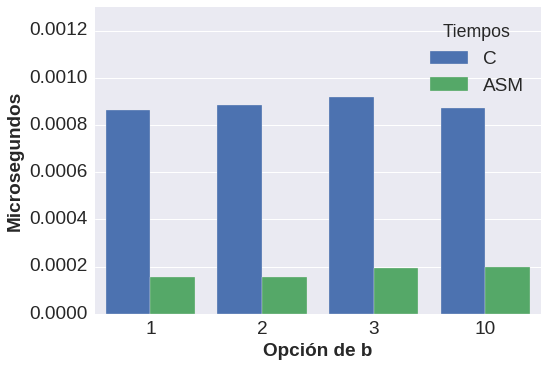
\includegraphics[width=70mm]{barplot_set_bnd_16_full_b_gcc_0}}
\subfigure[Promedios para tamaño 512x512.]{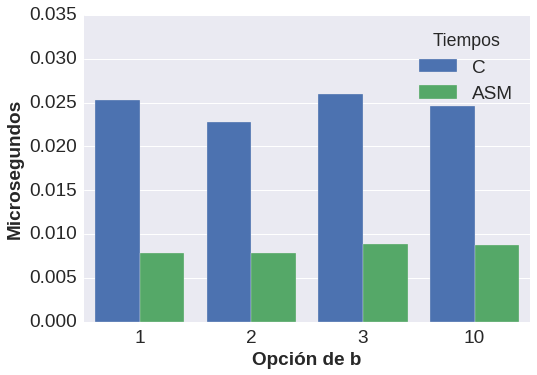
\includegraphics[width=70mm]{bar_plot_solver_set_bnd_512_full_b_gcc0}}  

\caption{Promedios podados de tiempo de ejecución para función $Solver Set Bnd$ sobre distintas implementaciones al variar parámetro $b$ sobre las cuatro opciones.} \label{fig:lego}
\end{figure}



Se muestra en Figura 3$(a)$ promedio podado de tiempo gastado en ejecución de los códigos, donde para cada tamaño los códigos fueron ejecutados 100 veces.
 

\begin{figure}[htbp]
\centering

\subfigure[Compilación hecha con gcc en opción o0]{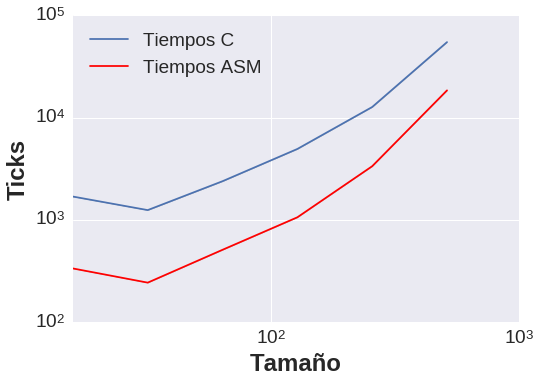
\includegraphics[width=120mm]{solver_set_bnd_0}}
\subfigure[Compilación hecha con gcc en opción o1]{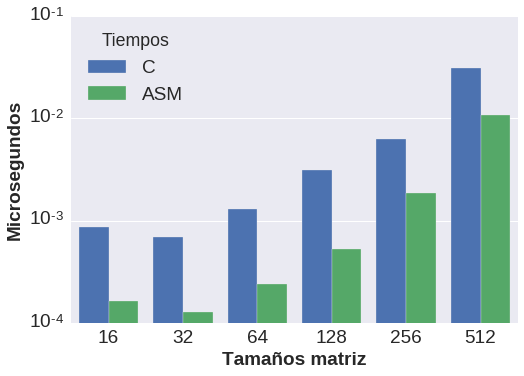
\includegraphics[width=70mm]{solver_set_bnd_1}}
\subfigure[Compilación hecha con gcc en opción o3]{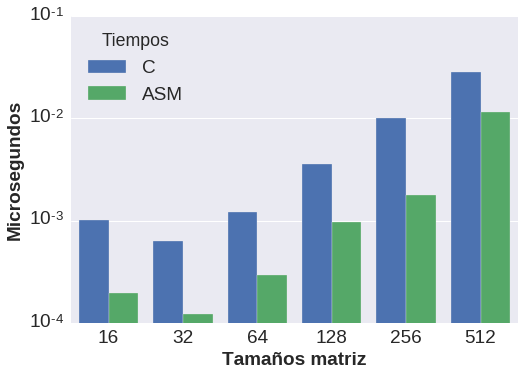
\includegraphics[width=70mm]{solver_set_bnd_3}} 

\caption{Promedios podados de tiempos de ejecución para función $Solver Set Bnd$ usando distintas opciones de optimización en compilador.} \label{fig:lego}
\end{figure}

Se ve que el código C gasta más tiempo que código ASM, achicándose esta diferencia a medida que aumenta el tamaño de matriz. Suponemos que esta ventaja de ASM sobre C se debe al uso de instrucciones SIMD en código ASM.

\subsubsection{Compilación hecha con gcc en opción o1}
Repetimos parámetros de función ($b$ en 1) para poder comparar las gráficas. El resultado se observa en Figura 3$(b)$.
 
No se nota mejora en tiempos C, ambas gráficas, la de $Solver Set Bnd$ y $gcc$ en $o0$ junto a la de $Solver Set Bnd$ y $gcc$ en $o1$, muestran comportamientos similares.

\subsubsection{Compilación hecha con gcc en opción o3}
Usamos mismas opciones de $b$ que para anteriores mediciones, $b$ en 1. El resultado se muestra en Figura 3$(c)$.
 
No vemos mejora en tiempos C, variando apenas los tiempos de este código a favor y en contra. 
\\

La función $Solver Set Bnd$ presenta buena diferencia en tiempos de ejecución, la implementación C tiende a tardar alrededor de seis veces el tiempo gastado por la implementación en ASM en nuestros experimentos. En este caso se utilizan instrucciones SIMD y no hay llamadas a las otras funciones.

 
\subsection{Función Solver Lin Solve}

\subsubsection{Compilación hecha con gcc en opción o0}
En este caso hemos variado los parámetros $a,b$ y $c$ solamente para tamaños de matriz 16x16 y 512x512. En la Figura 4 se muestran los promedios obtenidos para $1erOp$, $2daOp$, $3raOp$ y $4taOp$ sobre ambos tamaños. 
Para tamaño 16x16 (Figura 4(a)) en caso $1erOp$ debemos aclarar que porcentaje de datos no outliers es del 49$\%$ pero 61$\%$ restante se reparte un 30$\%$ arriba y otro 30$\%$ abajo de los no outliers, y por lo tanto este 49$\%$ refleja el comportamiento de la mayoría de los datos. Por otra parte destacamos caso $2daOp$, donde se observa pobre ventaja de código ASM, de alrededor del 10$\%$, sobre código C mientras que en los otros casos se obtiene un porcentaje de ventaja a favor de ASM levemente mayor. El desvío estandar obtenido indica datos poco dispersos respecto a la media, y el porcentaje de datos promediados (no outliers) está arriba del 60$\%$ para tiempos ASM y C, salvo caso señalado antes. A causa de esto decidimos aceptar al promedio como representación de la mayoría de los datos. Se observa misma comportamiento para 512x512 (Figura 4(b)) que para 16x16, con pobre ventaja para caso $2daOp$. A causa de esto hemos decidido evaluar la función usando $2daOp$ para todos los tamaños propuestos.
 
 \begin{figure}[htbp]
\centering

\subfigure[Promedios para tamaño 16x16.]{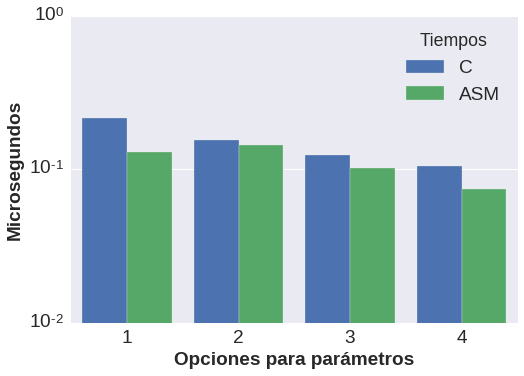
\includegraphics[width=70mm]{barplot_lin_solve_16_full_op}}
\subfigure[Promedios para tamaño 512x512.]{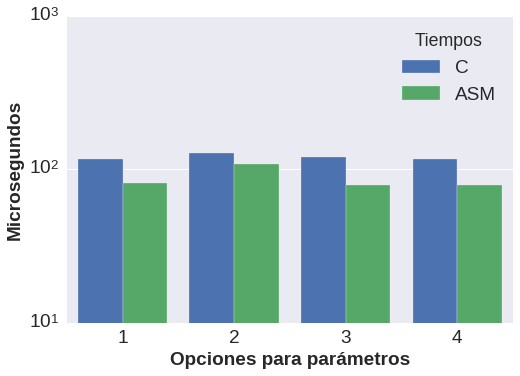
\includegraphics[width=70mm]{barplot_lin_solve_512_full_op}}  

\caption{Promedios podados de tiempo de ejecución para función $Solver Lin Solve$ sobre distintas implementaciones al variar parámetros sobre las cuatro opciones.} \label{fig:lego}
\end{figure}

Con parámetros de $2daOp$ variamos el tamaño de las matrices y graficamos los tiempos (ver Figura 5$(a)$).
  

\begin{figure}[htbp]
\centering

\subfigure[Compilación hecha con gcc en opción o0]{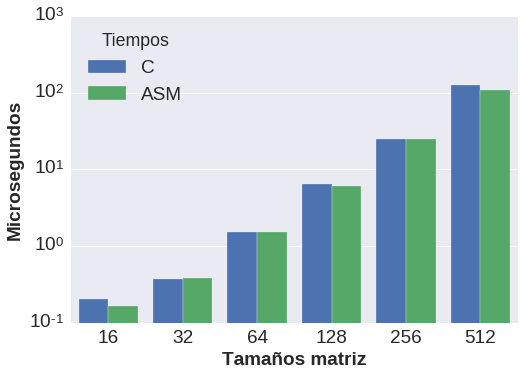
\includegraphics[width=120mm]{solver_lin_solve_0}}
\subfigure[Compilación hecha con gcc en opción o1]{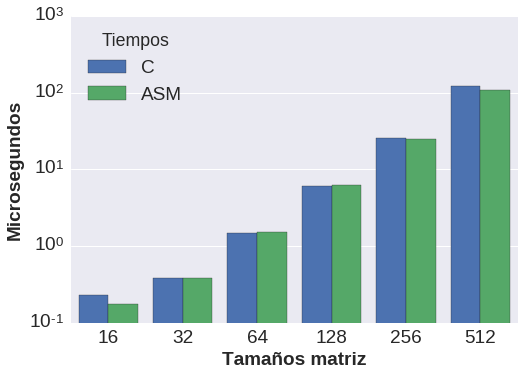
\includegraphics[width=70mm]{solver_lin_solve_1}}
\subfigure[Compilación hecha con gcc en opción o3]{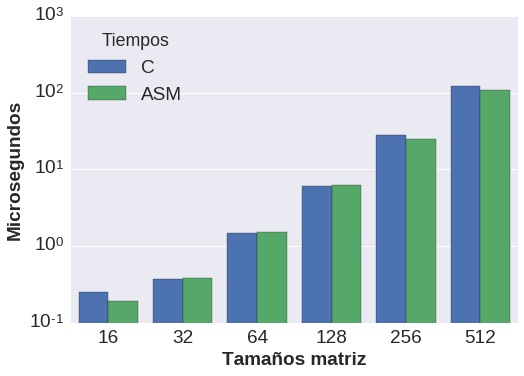
\includegraphics[width=70mm]{solver_lin_solve_3}} 

\caption{Promedios podados de tiempos de ejecución para función $Solver Lin Solve$ sobre distintas implementaciones.} \label{fig:lego}
\end{figure}

Se observa comportamiento similar de tiempo de ejecución, con código C apenas gastando más tiempo en tamaños arriba de 64x64 que ASM.
Suponemos que este comportamiento parejo es a causa de que si bien se usa instrucciones SIMD en código ASM no se aprovecha del todo el proceso de datos en paralelo a causa de restricciones de código C de la función, que es la fuente de implementación ASM.


\subsubsection{Compilación hecha con gcc en opción o1}
Para comparar gráficas hemos decidido repetir las mediciones con los mismos parámetros que usamos en anterior medición ($a, b$ y $c$ de $2daOp$). El resultado se ve en Figura 5(b).
 
No se ve una gran diferencia en los tiempos C y ASM manteniendose el comportamiento similar de gasto temporal al crecer en tamaño las matrices que usa la función.
  
\subsubsection{Compilación hecha con gcc en opción o3}
Repetimos parámetros de la función y graficamos los tiempos para distintos tamaños (Figura 5(c)).
 
Se ve que no hay cambios respecto a gráfica hecha con $gcc$ en opción $o0$ y $o1$. \\

La función $Solver Lin Solve$ presenta ínfima diferencia en tiempo de ejecución. Código C presentó un incremento en tiempo de ejecución de alrededor del 10$\%$ gastado por código ASM en el peor de los casos estudiados. Suponemos que la llamada a otra función influencia en la disminución de diferencia de tiempos pero sobre todo esto se debe a la restricción que hace el código fuente, C, a la implementación ASM, es decir la imposibilidad de procesar múltiples datos en paralelo aunque por lo menos logramos aprovechar las funciones SIMD al cargar múltiples datos de memoria en los registros XMM. Suponemos que la implementación en lenguaje C hace más accesos a memoria mirando la programación.

 
\subsection{Función Solver Project}

\subsubsection{Compilación hecha con gcc en opción o0} 
Se evalúan matrices con tamaño 16x16 y 512x512 sobre $1erOp$, $2daOp$, $3erOp$ y $4taOp$ para observar si hay gran cambio en las proporciones de tiempo al ejecutar código. Se observa en Figura 6 los resultados y se ve que para tamaño 16x16 implementación C tiende a gastar alrededor de 50$\%$ más de tiempo que código ASM.
El desvío estandar obtenido indica que los datos se mantienen cercanos a la media y el porcentaje de no outliers queda arriba del 60$\%$. En caso 512x512 (Figura 6(b)) se observa que C también tiende a gastar arriba de 60$\%$ más del total que gasta ASM, aunque los tiempos se muestran similares para todos los casos. Suponemos esto a causa de los altos tiempos de ejecución, que para tamaño 16x16 eran bajos, y entonces no se diferencian entre un caso y otro. El porcentaje de datos y el desvío estandar indican comportamiento similar a caso 16x16, más del 60$\%$ no outliers y datos cercanos a la media. Esto nos da confianza de tomar al promedio podado como representante de datos.
  
 \begin{figure}[htbp]
\centering

\subfigure[Promedios para tamaño 16x16.]{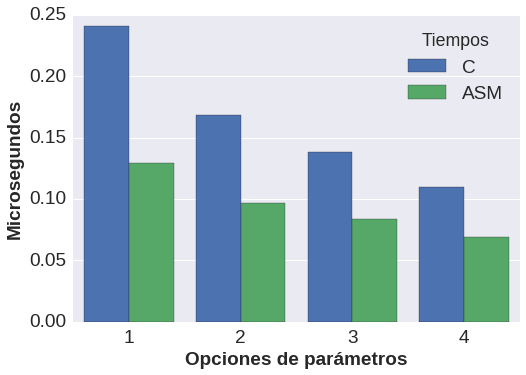
\includegraphics[width=70mm]{barplot_project_16_full_op}}
\subfigure[Promedios para tamaño 512x512.]{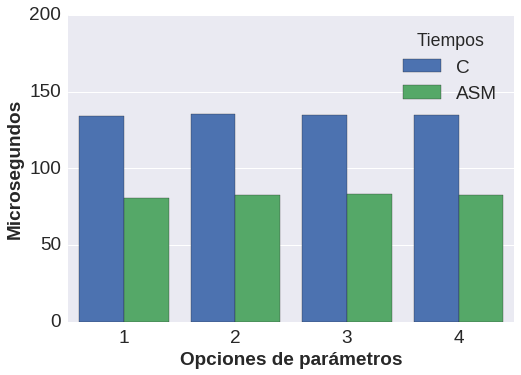
\includegraphics[width=70mm]{barplot_project_512_full_op}}  

\caption{Promedios podados de tiempo de ejecución para función $Solver Project$ sobre distintas implementaciones al variar parámetros sobre las cuatro opciones.} \label{fig:lego}
\end{figure}

A causa de este análisis hemos decidido usar matrices de caso $1erOp$ para evaluar la función. En la gráfica se muestran los promedios para distintos tamaños (Figura 7$(a)$).

%\begin{figure}[h]

%\centering
%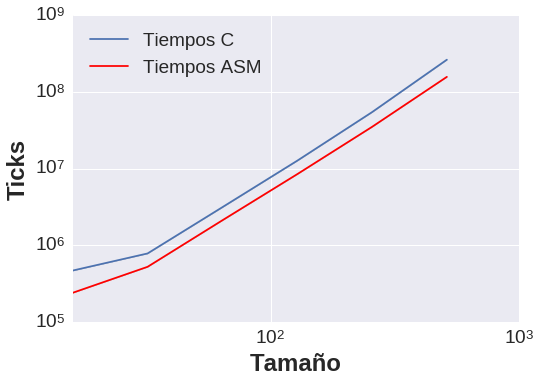
\includegraphics[scale=0.6] {solver_project_0}
 %  \caption{Tiempos en ticks de ejecución de código C vs código ASM para función solver project y gcc con opción o0}
%\end{figure}

\begin{figure}[htbp]
\centering

\subfigure[Compilación hecha con gcc en opción o0]{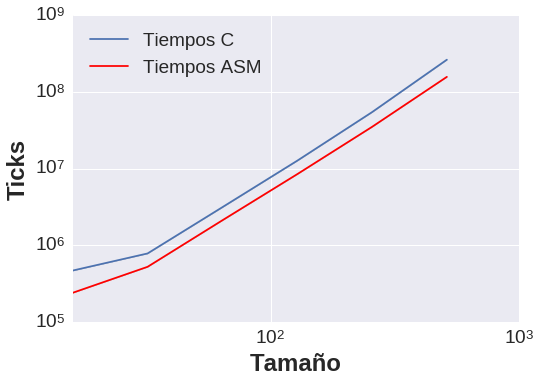
\includegraphics[width=70mm]{solver_project_0}}
\subfigure[Compilación hecha con gcc en opción o1]{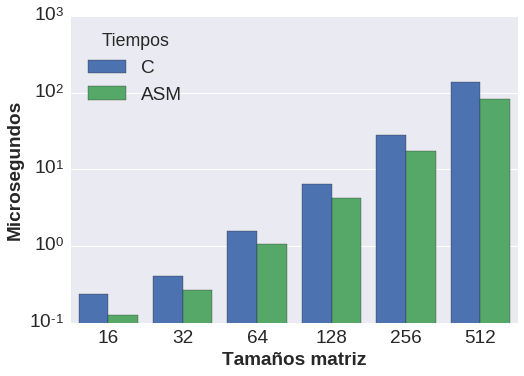
\includegraphics[width=70mm]{solver_project_1}}
\subfigure[Compilación hecha con gcc en opción o3]{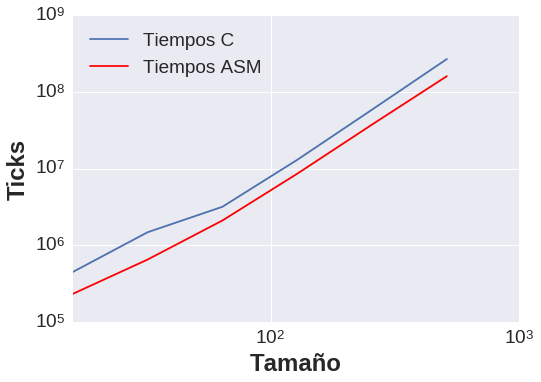
\includegraphics[width=70mm]{solver_project_3}} 

\caption{Promedio podado de tiempos de ejecución para función Solver Project.} \label{fig:lego}
\end{figure}

Se observa leve ventaja de tiempos de código ASM sobre código C. 
Suponemos que la llamada que hace $Solver Project$ a la función $Solver Lin Solve$ reduce la ventaja de código ASM sobre C ya que función $Solver Lin Solve$ mostró ínfima ventaja en algunos casos.


\subsubsection{Compilación hecha con gcc en opción o1}
Se usa misma selección de parámetros que en anterior medición, matrices de caso $1erOp$. En la Figura 7$(b)$ se ve el resultado.
 
Nuevamente no se nota cambios entre tiempos compilados con $gcc$ opción $o0$ y $gcc$ opción $o1$. 


\subsubsection{Compilación hecha con gcc en opción o3}
Repetimos parámetros en medición y obtuvimos el resultado de Figura 7$(c)$.
 
No se nota mejora en tiempos respecto a la de $Solver Project$ y $gcc$ en $o1$ y la de $Solver Project$ y $gcc$ en $o0$.
\\


La función $Solver Project$ presenta leve diferencia en tiempos de ejecución, implementación C tiende a tardar alrededor de un 50$\%$ más de tiempo que código ASM en nuestras mediciones. En este caso no se restringe el proceso múltiple de datos en la función y aprovechamos las funciones SIMD.

